\documentclass[letterpaper, reqno,11pt]{article}
\usepackage[margin=1.0in]{geometry}
\usepackage{color,latexsym,amsmath,amssymb,graphicx,float,listings,tikz}
\usepackage{hyperref}

\hypersetup{
colorlinks=true,
linkcolor=magenta,
filecolor=magenta,
urlcolor=cyan,
}

\lstset{
  basicstyle=\ttfamily,
  columns=fullflexible,
  frame=single,
  breaklines=true,
  postbreak=\mbox{\textcolor{red}{$\hookrightarrow$}\space},
}

\graphicspath{ {images/} }

\begin{document}
\pagenumbering{arabic}
\title{Homework }
\date{24/10/23}
\author{Xander Naumenko}
\maketitle

{\medskip\noindent\bf Question 1a.} All the code for question 1 will be shown at the end, so see there for the code used. For forward euler $G=1+z$ and for improved euler $G=1+z+\frac{z^2}{2}$, where $z=\Delta t\lambda=h\left( -1-\sqrt{3}i \right) $. The methods are stable when $|G|\leq 1$, and we can find when this is the case by numerically stepping $h$ until $G$ is no longer $\leq 1$. Specifically, I found that $h_m=0.05$ for Euler's method and $h_m=0.1$ for implicit Euler. The question is somewhat unclear on what is required by "solve the problem," but plots can be seen in figure \ref{fig:q1a} with the steps taken by $h>h_m,h=h_m$ and $h<h_m$. As expected, the larger the step size the more wild oscillation there is, indicating it doesn't converge outside the stability region. At $h=h_m$ the solution oscillates, while for $h<h_m$ the solution converges.

\begin{figure}[htpb]
    \centering
    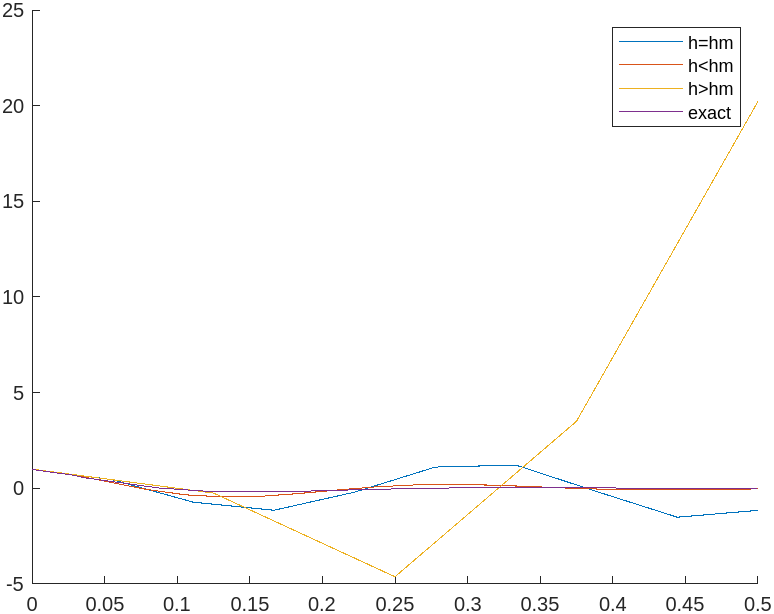
\includegraphics[width=0.8\textwidth]{q1aFE}
    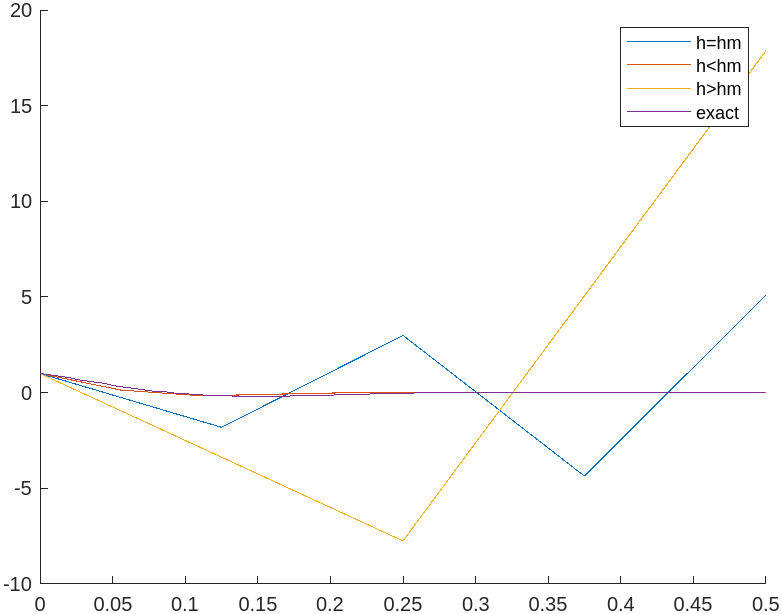
\includegraphics[width=0.8\textwidth]{q1aImpE}
    \caption{Graphs for question 1. Euler is on top and improved euler is on the bottom.}
    \label{fig:q1a}
\end{figure}

{\medskip\noindent\bf Question 1b.} Assume that $E(h)=ch^{p}$, we get
\[
Q=\log_2 \frac{E(h)}{E(h /2)}=\log_2 \frac{h^{p}}{(h /2)^{p}}=\log_2 2^{p}=p
.\]
To construct the table, each of the different methods were used to approximate the pde with the given step sizes. The resulting table can be seen in table \ref{tab:q1b}. As expected, in all cases $Q$ matches the order of the method.

\begin{table}
    \centering
    \begin{tabular}{|l|c|c|c|}
        \hline
        Method & $h = 2^{-2}$ & $h = 2^{-3}$ & $h = 2^{-4}$ \\
        \hline
        $E_{FE}$   & 0.109742974137801 & 0.055755448142280 & 0.028129665944480 \\
        $Q_{FE}$   & N/A                & 0.976943889897576 & 0.987020364888711 \\
        $E_{ImpE}$ & 0.009134808047836 & 0.002182768577992 & 0.000532085055283 \\
        $Q_{ImpE}$ & N/A                & 2.065215232753551 & 2.036430392572890 \\
        $E_{TR}$   & 0.004189470175650 & 0.001038640725659 & 0.000259127227082 \\
        $Q_{TR}$   & N/A                & 2.012071103505265 & 2.002964184676539 \\
        $E_{RK4}$  & 0.000012441224711 & 0.000000810387335 & 0.000000052122400 \\
        $Q_{RK4}$  & N/A                & 3.940373073325222 & 3.958636214804816 \\
        $E_{BE}$   & 0.118975470821564 & 0.058043829333979 & 0.028700539113078 \\
        $Q_{BE}$   & N/A                & 1.035449556899529 & 1.016064864826538 \\
        \hline
    \end{tabular}
    \caption{Your Table Caption Here}
    \label{tab:q1b}
\end{table}

Here is the code used for question 1:
\begin{lstlisting}
a=0;b=1;
f=@(x,y) x./(1.+x.^2).*y;
y0=1;
yexact = @(x) (1+x^2)^(1/2);

method = {@euler, @impEuler, @trapRule, @RK4, @BackEuler};
h=[2^(-2),2^(-3),2^(-4)];
T = zeros(10,3);
for i=1:5
   m = method{i};
   for j=1:3
      [X,Y] = feval(m,a,b,y0,(b-a)/h(j),f);
      T(i*2-1,j)=abs((yexact(1)-Y(1,end)));
      if j>1
         T(i*2,j)=log(T(i*2-1,j-1)/T(i*2-1,j))/log(2);
      end
   end
end

disp(T)

return

a=0;b=1/2;
f=@(x,y) 10*(-1-3^(1/2)*1i).*y;
y0=1;

% for h=[2^(-2), 2^(-3), 2^(-4)]
% h = 2^(-10);

h= 0;
lambda = 10*(-1-3^(1/2)*1i);
% while abs(1+h*lambda+(h*lambda)^2/2)<=1
while abs(1+h*lambda)<=1
   h=h+0.001;
end
disp(h)
% [Xm,Ym] = impEuler(a,b,y0,floor((b-a)/h),f);
% [Xs,Ys] = impEuler(a,b,y0,floor((b-a)/(h/2)),f);
% [Xb,Yb] = impEuler(a,b,y0,floor((b-a)/(h*2)),f);
[Xm,Ym] = euler(a,b,y0,floor((b-a)/h),f);
[Xs,Ys] = euler(a,b,y0,floor((b-a)/(h/2)),f);
[Xb,Yb] = euler(a,b,y0,floor((b-a)/(h*2)),f);
Xr = a:(b-a)/100:b;
Yr = exp(10*(-1-3^(1/2)*1i).*Xr);
hold on;
plot(Xm,Ym, "DisplayName", "h=hm");
plot(Xs,Ys, "DisplayName", "h<hm");
plot(Xb,Yb, "DisplayName", "h>hm");
plot(Xr,Yr, "DisplayName", "exact");
legend();
hold off;
% end

function [X,Y]=euler(a,b,y0,N,fun)
   h=(b-a)/N;
   X=a:h:b;Y(:,1)=y0;
   for i=1:N
      Y(:,i+1)=Y(:,i)+h*feval(fun,X(i),Y(:,i));
   end
end

function [X,Y]=impEuler(a,b,y0,N,fun)
   h=(b-a)/N;
   X=a:h:b;Y(:,1)=y0;
   for i=1:N
      Yt=Y(:,i)+h*feval(fun,X(i),Y(:,i));
      Y(:,i+1)=Y(:,i)+h/2*(feval(fun,X(i),Y(:,i))+feval(fun,X(i+1),Yt));
   end
end

function [X,Y]=trapRule(a,b,y0,N,fun)
h=(b-a)/N;hh=h/2;m=length(y0);
ep=sqrt(eps);maxit=15;I=eye(m);tol=1e-8;
X=a:h:b;Y(:,1)=y0;
   for i=1:N
      Y1 = Y(:,i); %+ h*feval(fun,X(i),Y(:,i));
      % Y1 = Y(:,i) + hh*(feval(fun,X(i),Y(:,i))+feval(fun,X(i)+h,Y1));
      R1 = (Y1 - Y(:, i) - h/2*(feval(fun, X(i)+h,Y1)+feval(fun,X(i),Y(:,i))));
      for it = 1:maxit 
        for j = 1:m
          D(:,j) = (feval(fun,X(i)+h,Y1+ep*I(:,j))-feval(fun,X(i)+h,Y1-ep*I(:,j)))/(2*ep);
        end
        J  = I - h*D;
        dY = -J\R1;
        Y1 = Y1 + dY;
        R1 = (Y1 - Y(:, i) - h/2*(feval(fun, X(i)+h,Y1)+feval(fun,X(i),Y(:,i))));
        RS(it)=norm(R1,2);
        if norm(R1,2) < tol*norm(Y1,2);break;end
      end
      %plot(1:it,log10(RS));pause;RS=[];
      if it >=maxit,
          msg=[' WARNING: in step ',num2str(i),' Newton Iteration did not converge in ',num2str(maxit),' iterations ']
      end
      Y(:,i+1)=Y(:,i)+hh*(feval(fun,X(i)+h,Y1)+feval(fun,X(i),Y(:,i)));
   end
end

function [X,Y]=RK4(a,b,y0,N,fun)
h=(b-a)/N;hh=h/2;m=length(y0);
ep=sqrt(eps);maxit=15;I=eye(m);tol=1e-8;
X=a:h:b;Y(:,1)=y0;
   for i=1:N
      Y1 = Y(:,i); %+ h*feval(fun,X(i),Y(:,i));
      % Y1 = Y(:,i) + hh*(feval(fun,X(i),Y(:,i))+feval(fun,X(i)+h,Y1));
      R1 = (Y1-Y(:,i)-h*feval(fun,X(i)+h,Y1));
      for it = 1:maxit 
        for j = 1:m
          D(:,j) = (feval(fun,X(i)+h,Y1+ep*I(:,j))-feval(fun,X(i)+h,Y1-ep*I(:,j)))/(2*ep);
        end
        J  = I - h*D;
        dY = -J\R1;
        Y1 = Y1 + dY;
        R1 = (Y1-Y(:,i)-h*feval(fun,X(i)+h,Y1));
        RS(it)=norm(R1,2);
        if norm(R1,2) < tol*norm(Y1,2);break;end
      end
      %plot(1:it,log10(RS));pause;RS=[];
      if it >=maxit,
          msg=[' WARNING: in step ',num2str(i),' Newton Iteration did not converge in ',num2str(maxit),' iterations ']
      end
      m1=feval(fun,X(i),Y(:,i));
      m2=feval(fun,X(i)+h/2,Y(:,i)+h/2*m1);
      m3=feval(fun,X(i)+h/2,Y(:,i)+h/2*m2);
      m4=feval(fun,X(i)+h,Y(:,i)+h*m3);
      Y(:,i+1)=Y(:,i)+h/6*(m1+2*m2+2*m3+m4);
   end
end

function [X,Y]=BackEuler(a,b,y0,N,fun)
h=(b-a)/N;hh=h/2;m=length(y0);
ep=sqrt(eps);maxit=15;I=eye(m);tol=1e-8;
X=a:h:b;Y(:,1)=y0;
   for i=1:N
      Y1 = Y(:,i); %+ h*feval(fun,X(i),Y(:,i));
      %Y1 = Y(:,i) + hh*(feval(fun,X(i),Y(:,i))+feval(fun,X(i)+h,Y1));
      R1 = (Y1-Y(:,i)-h*feval(fun,X(i)+h,Y1));
      for it = 1:maxit 
        for j = 1:m
          D(:,j) = (feval(fun,X(i)+h,Y1+ep*I(:,j))-feval(fun,X(i)+h,Y1-ep*I(:,j)))/(2*ep);
        end
        J  = I - h*D;
        dY = -J\R1;
        Y1 = Y1 + dY;
        R1 = (Y1-Y(:,i)-h*feval(fun,X(i)+h,Y1));
        RS(it)=norm(R1,2);
        if norm(R1,2) < tol*norm(Y1,2);break;end
      end
      %plot(1:it,log10(RS));pause;RS=[];
      if it >=maxit,
          msg=[' WARNING: in step ',num2str(i),' Newton Iteration did not converge in ',num2str(maxit),' iterations ']
      end
      Y(:,i+1)=Y(:,i)+h*feval(fun,X(i)+h,Y1);
   end
end
\end{lstlisting}

% {\medskip\noindent\bf Question 2a.} Calculating the truncation error:
% \[
% T_n(\Delta t)= \frac{y_{n+2}-y_n}{\Delta t}- \frac{1}{2}\left( f(t_{n+1},y_n+\Delta t)+ \right) 
% .\]
{\medskip\noindent\bf Question 2a.} Considering the model problem $\dot y=\lambda y$ (this isn't strictly rigorous but was shown in class so I assume it's fine):
\[
T_k(h)=\frac{y_{k+2}-y_k}{h}-\frac{1}{2}(\lambda(y_{k}+h\lambda y_k)+3\lambda y_k)
\]
\[
=\frac{y_k+2h\dot y_k+ 2h^2\ddot y_k+ \frac{4}{3}h^3\dddot y_k+\ldots-y_k}{h}-(2\lambda y_k+\frac{\lambda^2}{2}h y_k)
\]
\[
=\frac{3}{2}\lambda^2h+\ldots=O(h)
.\]

Thus the difference scheme has local truncation error $O(h)$.

{\medskip\noindent\bf Question 2b.} Substituting $Y_k=G^{k}$:
\[
G^{k+2}=G^{k}+\frac{h}{2}\left( \lambda G^{k+1}+3\lambda G^{k} \right) \implies 2G^2-2=z(G+3)\implies 2G^2-zG-3z-2=0
.\]
Substituting $G=e^{i\theta}$ gives:
\[
z=\frac{2e^{2i\theta}-2}{e^{i\theta}+3}
.\]
Plotting this, we can see in figure \ref{fig:q2b} that the stability region boundary is that of a circle, with the inside being stable. The code used to generate it is:
\begin{lstlisting}
theta = 0:0.01:2*pi;

z=(2.*exp(2i.*theta)-2)./(exp(1i.*theta)+3);

plot(real(z),imag(z));
axis equal;
grid on;
xlabel("Re(z)");
ylabel("Im(z)");
\end{lstlisting}

\begin{figure}[htpb]
    \centering
    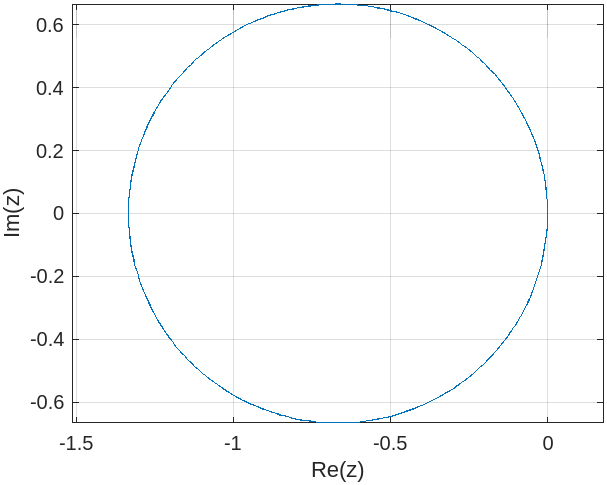
\includegraphics[width=0.8\textwidth]{q2b}
    \caption{Stability region for question 2. Inside is stable.}
    \label{fig:q2b}
\end{figure}

{\medskip\noindent\bf Question 3a.} See figure \ref{fig:q3a}, as previously the code used to generate all the plots is at the end of this question. Note that implicit Euler was left off the plot, as it diverges and causes the other methods not to be seen. The reason it diverges is that the initial slope $y'(0)$ it sees is extremely large ($-1000(1-0)+1=-999)$), so this sends it off extremely far on the first time step, thus effectively throwing off the initial conditions completely. Backwards euler is almost completely immune to this, and it matches the exact solution almost precisely. The reason for this is that it explicitly doesn't even consider $f(0,y(0))$ in the difference equation, so a large outlier value at the beginning has no effect. Crank-Nicolson/trapezium is somewhere in the middle, with the large value at the beginning throwing the solution off and causing it to oscillate (Since $|z|> >2\implies G=\frac{2+z}{2-z}\approx -1$), but not so much as for improved Euler where it diverges.

\begin{figure}[htpb]
    \centering
    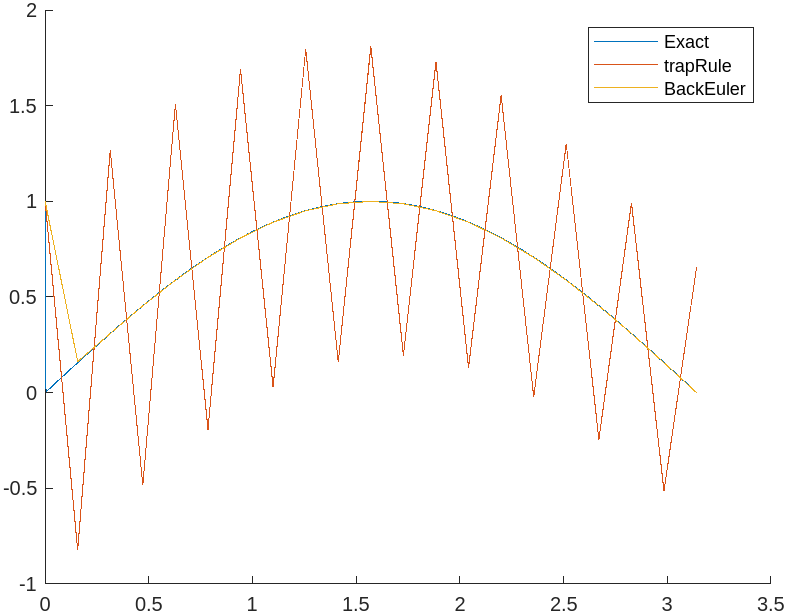
\includegraphics[width=0.8\textwidth]{q3a}
    \caption{Plot for question 3a. Note that improved Euler was left off this plot as it diverges and hides the other methods.}
    \label{fig:q3a}
\end{figure}

{\medskip\noindent\bf Question 3b.} Ignoring the non-homogenous terms, we can consider $\lambda=-1000$ and solve the equation $G=1+z+\frac{1}{2}z^2$ where $z=\lambda h$. Since $\lambda$ is real then the maximum stable $h$ will come when $G=1$, i.e.
\[
1=1-1000h+500000h^2\implies h=\frac{1}{500}
.\]
Numerically trying this, we get the plot seen in figure \ref{fig:q3b} using step size of exactly $h=\frac{1}{500}$, which corresponds to 1571 steps. Note that although not matching the exact solution, it does at least converge. I also tried step size of $h=\frac{1}{499}$ and $h=\frac{1}{501}$, and indeed $h=\frac{1}{499}$ diverges while $h=\frac{1}{501}$ converges noticeably more accurately than $h=\frac{1}{500}$ (it doesn't hover over the exact solution).

\begin{figure}[htpb]
    \centering
    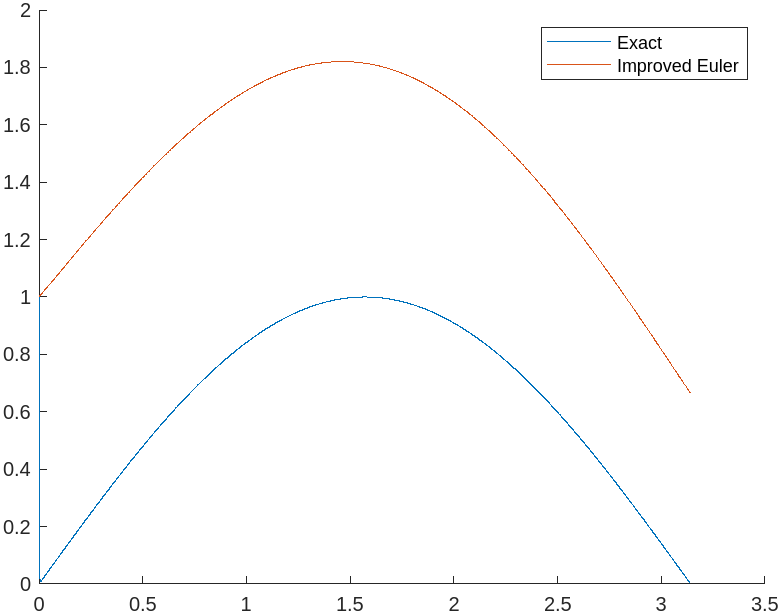
\includegraphics[width=0.8\textwidth]{q3b}
    \caption{Plot for question 3b.}
    \label{fig:q3b}
\end{figure}

{\medskip\noindent\bf Question 3c.} See figure \ref{fig:q3c} for the plot. ode23 required 1264 sample points to solve the system. This is obviously a lot better than forward Euler which took 1574 steps to even converge. The main conclusion from this exercise is that you have to be very around stiff ODEs when numerically simulating them, as they are very sensitive to the method used. Despite the superficial similarities of improved euler vs. backwards euler, they behave completely different convergence requirements when used here.

Here is the code used for question 3:

\begin{figure}[htpb]
    \centering
    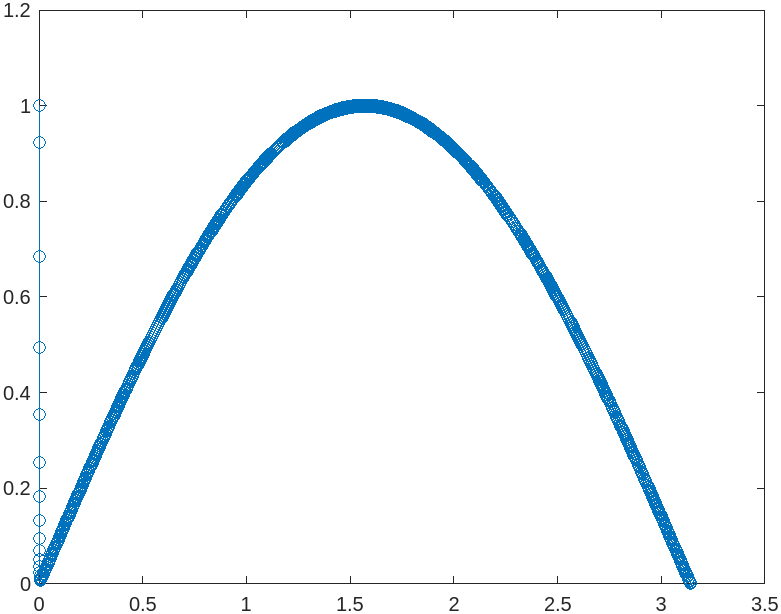
\includegraphics[width=0.8\textwidth]{q3c}
    \caption{Plot for question 3c.}
    \label{fig:q3c}
\end{figure}
\begin{lstlisting}
alpha=1000;
a=0;b=pi;
f=@(x,y) -alpha*(y-sin(x))+cos(x);
y0=1;
N=20;
sol = @(x) sin(x)+exp(-alpha*x);

[X,Y] = ode23(f,[a,b],y0,odeset('AbsTol',0.0001));

plot(X,Y,'-o');
disp(size(X))

return

hold on;
X = a:0.001:b;
Y = sol(X);
plot(X,Y,"DisplayName",'Exact');

[Xe, Ye] = impEuler(a,b,y0,ceil((b-a)/(1/500)),f);
plot(Xe,Ye,"DisplayName",'Improved Euler');
hold off;
legend();

return

method = {@trapRule, @BackEuler};
hold on;
X = a:0.001:b;
Y = sol(X);
plot(X,Y,"DisplayName",'Exact');
for i=1:2
   m = method{i};
   [X,Y] = m(a,b,y0,N,f);
   plot(X,Y,"DisplayName",char(m));
end
hold off;
legend();

function [X,Y]=impEuler(a,b,y0,N,fun)
   h=(b-a)/N;
   X=a:h:b;Y(:,1)=y0;
   for i=1:N
      Yt=Y(:,i)+h*feval(fun,X(i),Y(:,i));
      Y(:,i+1)=Y(:,i)+h/2*(feval(fun,X(i),Y(:,i))+feval(fun,X(i+1),Yt));
   end
end

function [X,Y]=trapRule(a,b,y0,N,fun)
h=(b-a)/N;hh=h/2;m=length(y0);
ep=sqrt(eps);maxit=15;I=eye(m);tol=1e-8;
X=a:h:b;Y(:,1)=y0;
   for i=1:N
      Y1 = Y(:,i); %+ h*feval(fun,X(i),Y(:,i));
      % Y1 = Y(:,i) + hh*(feval(fun,X(i),Y(:,i))+feval(fun,X(i)+h,Y1));
      R1 = (Y1 - Y(:, i) - h/2*(feval(fun, X(i)+h,Y1)+feval(fun,X(i),Y(:,i))));
      for it = 1:maxit 
        for j = 1:m
          D(:,j) = (feval(fun,X(i)+h,Y1+ep*I(:,j))-feval(fun,X(i)+h,Y1-ep*I(:,j)))/(2*ep);
        end
        J  = I - h*D;
        dY = -J\R1;
        Y1 = Y1 + dY;
        R1 = (Y1 - Y(:, i) - h/2*(feval(fun, X(i)+h,Y1)+feval(fun,X(i),Y(:,i))));
        RS(it)=norm(R1,2);
        if norm(R1,2) < tol*norm(Y1,2);break;end
      end
      %plot(1:it,log10(RS));pause;RS=[];
      if it >=maxit,
          msg=[' WARNING: in step ',num2str(i),' Newton Iteration did not converge in ',num2str(maxit),' iterations ']
      end
      Y(:,i+1)=Y(:,i)+hh*(feval(fun,X(i)+h,Y1)+feval(fun,X(i),Y(:,i)));
   end
end

function [X,Y]=BackEuler(a,b,y0,N,fun)
h=(b-a)/N;hh=h/2;m=length(y0);
ep=sqrt(eps);maxit=15;I=eye(m);tol=1e-8;
X=a:h:b;Y(:,1)=y0;
   for i=1:N
      Y1 = Y(:,i); %+ h*feval(fun,X(i),Y(:,i));
      %Y1 = Y(:,i) + hh*(feval(fun,X(i),Y(:,i))+feval(fun,X(i)+h,Y1));
      R1 = (Y1-Y(:,i)-h*feval(fun,X(i)+h,Y1));
      for it = 1:maxit 
        for j = 1:m
          D(:,j) = (feval(fun,X(i)+h,Y1+ep*I(:,j))-feval(fun,X(i)+h,Y1-ep*I(:,j)))/(2*ep);
        end
        J  = I - h*D;
        dY = -J\R1;
        Y1 = Y1 + dY;
        R1 = (Y1-Y(:,i)-h*feval(fun,X(i)+h,Y1));
        RS(it)=norm(R1,2);
        if norm(R1,2) < tol*norm(Y1,2);break;end
      end
      %plot(1:it,log10(RS));pause;RS=[];
      if it >=maxit,
          msg=[' WARNING: in step ',num2str(i),' Newton Iteration did not converge in ',num2str(maxit),' iterations ']
      end
      Y(:,i+1)=Y(:,i)+h*feval(fun,X(i)+h,Y1);
   end
end

\end{lstlisting}

{\medskip\noindent\bf Question 4a.} All three routines were converted to handle linked equations as the ones given. The plots of the trajectories can be seen in figure \ref{fig:q4a}. It is clear from the plots that Euler's method causes the radius to increase, the trapezoid rule preserves radius and backwards Euler shrinks it. Only in the trapezoid case is the circle perfectly reproduced. This is the code used for the plots:

\begin{figure}[htpb]
    \centering
    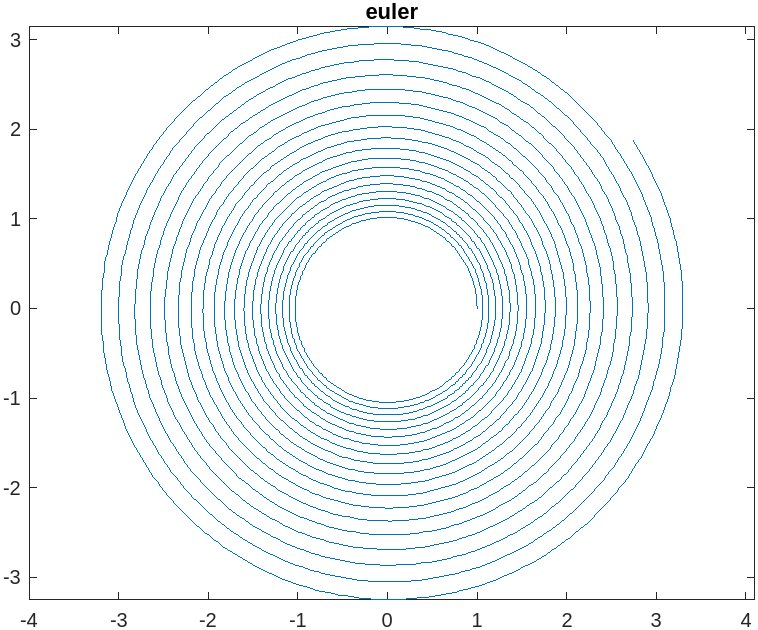
\includegraphics[width=0.4\textwidth]{q4a1}
    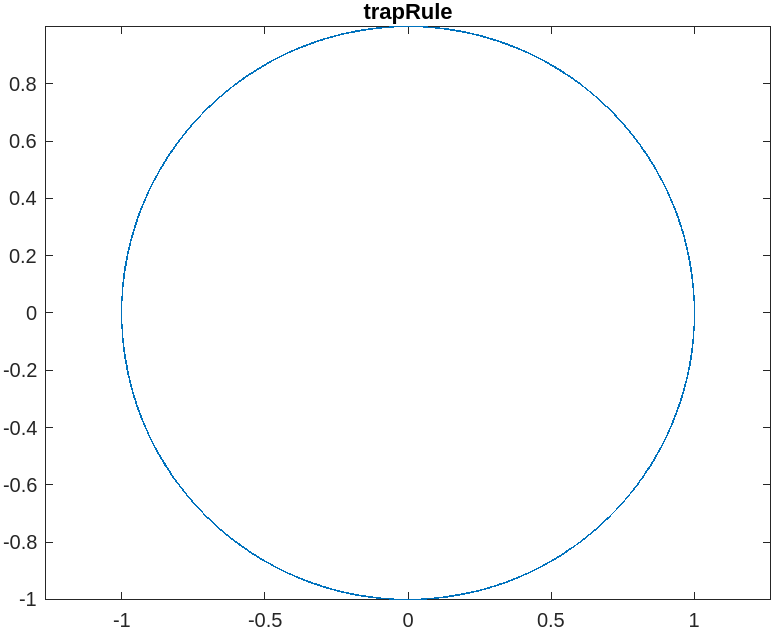
\includegraphics[width=0.4\textwidth]{q4a2}
    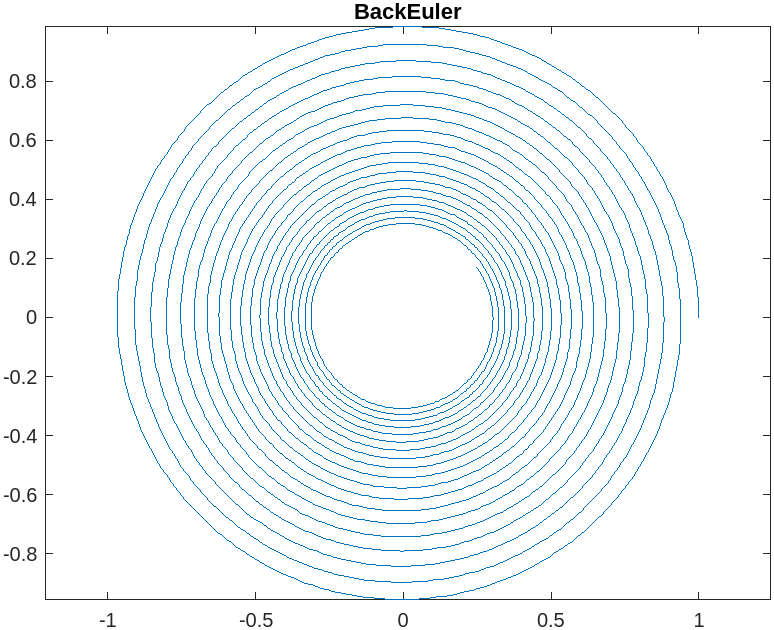
\includegraphics[width=0.4\textwidth]{q4a3}
    \caption{Graphs for question 4a.}
    \label{fig:q4a}
\end{figure}

\begin{lstlisting}
r = 1;
% fxr = @(theta,x) -r*sin(theta);
% fyr = @(theta,y) r*cos(theta);
fx = @(x,y) -y;
fy = @(x,y) x;
x0 = r;
y0 = 0;
h=0.02;
a=0;b=120;

method = {@euler, @trapRule, @BackEuler};
for i=1:3
   figure;
   m=method{i};
   N=(b-a)/h;
   [thetax,X,Y]=m(a,b,x0,y0,N,fx,fy);
   plot(X,Y);
   axis equal;
   title(char(m));
end

function [theta,X,Y]=euler(a,b,x0,y0,N,fx,fy)
   h=(b-a)/N;
   theta=a:h:b;X(:,1)=x0;Y(:,1)=y0;
   for i=1:N
      X(:,i+1)=X(:,i)+h*feval(fx,X(:,i),Y(:,i));
      Y(:,i+1)=Y(:,i)+h*feval(fy,X(:,i),Y(:,i));
   end
end

function [theta,X,Y]=trapRule(a,b,x0,y0,N,fx,fy)
   h=(b-a)/N;hh=h/2;m=length(y0);
   ep=sqrt(eps);maxit=15;I=eye(m);tol=1e-8;
   theta=a:h:b;X(:,1)=x0;Y(:,1)=y0;
   for i=1:N
     X1 = X(:,i);
     Y1 = Y(:,i);
     % R1 = (Y1 - Y(:, i) - h/2*(feval(fy, X(:,i)+h,Y1)+feval(fy,X(:,i),Y(:,i))));
     % R2 = (X1 - X(:, i) - h/2*(feval(fx, X(:,i),Y1+h)+feval(fx,X(:,i),Y(:,i))));
     R1 = (Y1 - Y(:, i) - h/2*(feval(fy, X1,Y1)+feval(fy,X(:,i),Y(:,i))));
     R2 = (X1 - X(:, i) - h/2*(feval(fx, X1,Y1)+feval(fx,X(:,i),Y(:,i))));
     for it = 1:maxit 
        for j = 1:m
          Dy(:,j) = (feval(fy,X1,Y1+ep*I(:,j))-feval(fy,X1,Y1-ep*I(:,j)))/(2*ep);
          Dx(:,j) = (feval(fx,X1+ep*I(:,j),Y1)-feval(fx,X1-ep*I(:,j),Y1))/(2*ep);
        end
        Jy  = I - h*Dy;
        Jx  = I - h*Dx;
        dY = -Jy\R1;
        dX = -Jx\R2;
        Y1 = Y1 + dY;
        X1 = X1 + dX;
        R1 = (Y1 - Y(:, i) - h/2*(feval(fy, X1,Y1)+feval(fy,X(:,i),Y(:,i))));
        R2 = (X1 - X(:, i) - h/2*(feval(fx, X1,Y1)+feval(fx,X(:,i),Y(:,i))));
        if norm([R1,R2],2) < tol*norm([Y1,X1],2);break;end
      end
      %plot(1:it,log10(RS));pause;RS=[];
      if it >=maxit,
          msg=[' WARNING: in step ',num2str(i),' Newton Iteration did not converge in ',num2str(maxit),' iterations ']
      end
      Y(:,i+1)=Y(:,i)+hh*(feval(fy,X1,Y1)+feval(fy,X(:,i),Y(:,i)));
      X(:,i+1)=X(:,i)+hh*(feval(fx,X1,Y1)+feval(fx,X(:,i),Y(:,i)));
   end
end

function [theta,X,Y]=BackEuler(a,b,x0,y0,N,fx,fy)
   h=(b-a)/N;hh=h/2;m=length(y0);
   ep=sqrt(eps);maxit=15;I=eye(m);tol=1e-8;
   theta=a:h:b;X(:,1)=x0;Y(:,1)=y0;
   for i=1:N
     X1 = X(:,i);
     Y1 = Y(:,i);
     % R1 = (Y1 - Y(:, i) - h/2*(feval(fy, X(:,i)+h,Y1)+feval(fy,X(:,i),Y(:,i))));
     % R2 = (X1 - X(:, i) - h/2*(feval(fx, X(:,i),Y1+h)+feval(fx,X(:,i),Y(:,i))));
     R1 = Y1 - Y(:, i) - h*feval(fy, X1,Y1);
     R2 = X1 - X(:, i) - h*feval(fx, X1,Y1);
     for it = 1:maxit 
        for j = 1:m
          Dy(:,j) = (feval(fy,X1,Y1+ep*I(:,j))-feval(fy,X1,Y1-ep*I(:,j)))/(2*ep);
          Dx(:,j) = (feval(fx,X1+ep*I(:,j),Y1)-feval(fx,X1-ep*I(:,j),Y1))/(2*ep);
        end
        Jy  = I - h*Dy;
        Jx  = I - h*Dx;
        dY = -Jy\R1;
        dX = -Jx\R2;
        Y1 = Y1 + dY;
        X1 = X1 + dX;
        R1 = Y1 - Y(:, i) - h*feval(fy, X1,Y1);
        R2 = X1 - X(:, i) - h*feval(fx, X1,Y1);
        if norm([R1,R2],2) < tol*norm([Y1,X1],2);break;end
      end
      %plot(1:it,log10(RS));pause;RS=[];
      if it >=maxit,
          msg=[' WARNING: in step ',num2str(i),' Newton Iteration did not converge in ',num2str(maxit),' iterations ']
      end
      Y(:,i+1)=Y(:,i)+h*feval(fy,X1,Y1);
      X(:,i+1)=X(:,i)+h*feval(fx,X1,Y1);
   end
end
\end{lstlisting}

{\medskip\noindent\bf Question 4b.} By multiplying by $x$ and $y$ respectively, we get the following set of equations:
\[
\begin{cases}
    x x'=-xy\\
    yy'=xy
\end{cases}
.\]
Adding them together and multiplying by 2, we get
\[
2\int x x'+y y' d\theta=x^2+y^2=2\int 0d\theta=r^2
\]
as expected. Starting with forward Euler, we can do something similar. The difference equation for forward Euler, multiplied in the same way as above is:
\[
\begin{cases}
    X_{n+1}X_{n+1}=X_{n+1}\left( X_n-hY_{n} \right) \\
    Y_{n+1}Y_{n+1}=Y_{n+1}\left( Y_n+hX_n \right) 
\end{cases}\implies \begin{cases}
    X_{n+1}^2=X_n(X_n-hY_n)-hY_n(X_n-hY_n)\\
    Y_{n+1}^2=Y_n\left( Y_n+hX_n \right) +hX_n\left( Y_n+hX_n \right) 
\end{cases}
\]
\[
\implies X_{n+1}^2+Y_{n+1}^2=h^2\left( X_{n}^2+Y_{n}^2 \right) +X_n^2+Y_n^2\implies R_{n+1}^2=R_n^2+h^2R_n^2
.\]
Thus, as seen in part a, the radius expands outwards. Next, for backwards Euler the picture is almost the exact same except in reverse:
\[
\begin{cases}
    X_{n+1}X_{n+1}=X_{n+1}\left( X_n-hY_{n+1} \right) \\
    Y_{n+1}Y_{n+1}=Y_{n+1}\left( Y_n+hX_{n+1} \right) 
\end{cases}\implies X_{n+1}^2+Y_{n+1}^2=X_nX_{n+1}+Y_nY_{n+1}=X_{n}^2+Y_n^2-h^2(X_{n+1}^2+Y_{n+1}^2)
\]
\[
\implies R_{n+1}^2=R_n^2-h^2R_{n+1}^2
.\]
Again, this matches what we saw in part a where the radius continuously got smaller for backwards Euler. Finally, for trapezoid:
\[
\begin{cases}
    X_{n+1}^2=X_nX_{n+1}-\frac{h}{2}X_{n+1}\left( Y_n+Y_{n+1} \right) \\
    Y_{n+1}^2=Y_nY_{n+1}+\frac{h}{2}Y_{n+1}\left( X_{n}+X_{n+1} \right) 
\end{cases}\implies X_{n+1}^2+Y_{n+1}^2=\frac{h}{2}\left( X_nY_{n+1}-Y_nY_{n+1} \right) X_nX_{n+1}+Y_nY_{n+1}
\]
Replacing the $n+1$ terms in the above with their definitions in the trapezoid scheme and rearrange, we arrive at
\[
\implies R_{n+1}^2=0
.\]
This also matches what we saw in part a, where the trapezoid scheme perfectly preserved radius.

\end{document}
